%tag: DD-Rev0
\documentclass[12,english]{article}
\usepackage[letterpaper, portrait, margin=1in]{geometry}

\usepackage{amsmath}
\usepackage[T1]{fontenc}
\usepackage{babel}
\usepackage{textcomp}
\usepackage{titlesec}
\setcounter{secnumdepth}{4}
\usepackage{hyperref}
\usepackage{xcolor}
\usepackage{booktabs}
\usepackage{placeins}
\usepackage{graphicx}
\usepackage{cite}

\usepackage{booktabs}
\usepackage{tabularx}
\usepackage{float}
\usepackage{cite}
%\usepackage[colorlinks,linkcolor=blue]{hyperref}
\usepackage{color}
\usepackage{ulem}

\graphicspath{ {images/} }


\titleformat{\paragraph}
{\normalfont\normalsize\bfseries}{\theparagraph}{1em}{}
\titlespacing*{\paragraph}
{0pt}{3.25ex plus 1ex minus .2ex}{1.5ex plus .2ex}

\title{Module Guide for Group 15 - FlightShootingGame}
\author{Yijun Chen\\
\texttt{ (cheny161)}
\and
Tianxing Li\\
\texttt{(lit20)}
\and
Zefeng Wang\\
\texttt{(wangz217)}
}

\date{}


\begin{document}
\maketitle
\newpage
\tableofcontents
\newpage

\section{Introduction}
	\subsection{Overview}
	The retro flight shooting game is the re-implementation of an open-source python game on Github. By using the Pyxel library, the game is interpreted in 8-bits graphic style, and the final version will be played on \sout{Python platform} {\color{red}devices with Python3 and Pyxel library installed}.
	\subsection{Context}
	This document is the Module Guide(MG) and the main purpose of it is to provide a modular decomposition of the system, showing the modular structure. The document is created after the Software Requirements Specification(SRS), which specifies all the functional and non-functional requirements for the project. Hence, MG specifies how the system meets both functional and non-functional requirements mentioned in the SRS. \cite{b2}

After the creation of the MG, as a part of Design Document the Module Interface Specification (MIS) is formed. The MIS explains the semantics (state and environment variables, assumptions, and access routines) and syntax of exported functions (input, output, and exceptions) for every module, providing additional detail on each module that was laid out in the MG.\cite{b2}
	\subsection{Design Principles}
	
	The Design Principles being used to guide the decomposition of the system into modules are Information Hiding and Encapsulation, as well as the principle that a Uses Relation (Hierarchy) should contain no cycles, have low coupling, and high cohesion. \cite{b2}

The principle of Information Hiding is that each module hides a secret (a design decision) from the rest of the system. The principle of Encapsulation is that changeable information is in the implementation of the module, but the module interface should not change when the implementation changes (the services it provides are accessed in a consistent way regardless of changes in implementation). Cycles in the Uses Relation means that module A uses module B, which uses module A. This is considered poor design because it can cause infinite loops and there is likely a better way to decompose the modules. Low coupling means that the modules are independent and do not use many other modules. High cohesion means that the elements within a module are strongly related.\cite{b2}
	\subsection{Document Structure}
	{\color{red}The document structure is organized as follows}:
\begin{itemize}

\item {\color{red}Section 2 lists Anticipated and Unlikely Changes to the system's implementation. This list is used for the Traceability Matrices later in the document.}

\item Section 3 details the Module Hierarchy, listing all the modules and their hierarchy by secrets. 

\item Section 4 explains the Connection Between Requirements and Design, which details how the software requirements are related to the modules. 

\item Section 5 provides the Module Decomposition, detailing the module name, secret, and service/responsibility for each module. 

\item Section 6 provides the Traceability Matrices. The first matrix connects the requirements to the modules, thereby checking completeness of the design against the requirements provided in the SRS. The second matrix connects anticipated changes from Section 2 to the modules.

\item Section 7 provides the Uses Hierarchy for the project, which shows the uses relations between modules.

\item Section 8 provides the Project Schedule for the rest of the term, providing Gantt chart.
\item Section 9 provides the Major Revision History for the document.
\end{itemize}	

\section{Anticipated and Unlikely Changes}

\subsection{Anticipated Changes}

AC1: The format of the input data.\\
AC2: The format of the input parameters.\\
AC3: The format of the output data.\\
AC4: How the frame rate is defined using the input parameters.\\
AC5: The graphical user interface elements used to retrieve user input and their format.\\
AC6: Default settings for input.\\
AC7: Parameters of enemy bullets. (i.e. speed, damage, etc.)\\
AC8: Moving route of enemy planes.

\subsection{Unlikely Changes}

UC1: Input/Output devices to the system (system assumes speaker, keyboard, and screen are available.)\\
UC2: The moving pattern of all enemies.\\
UC3: The frame rate can be defined by input parameters and data.\\
UC4: The storage method of output data. In this case, the only output data is the high score, which is stored in a .txt file.

\section{Module Hierarchy}

\begin{table}[!htbp]
        \begin{tabular}{ll}
        \toprule
        Level 1 & Level 2 \\
        \midrule
        Hardware Hiding Module & \\
         \midrule
        Behaviour Hiding Module & Boss Module \\%1
        & Bullet Module\\%2
        & Smart\_Bullet Module\\%3
        & Enemy Module, Player Module\\%4, 5
        & Gift Module\\%6
		& Music Module \\%7
		 \midrule
        Software Decision Module & \\
        \bottomrule
        \end{tabular}
        \caption{Module Hierarchy}
        % Colour for the rulings in tables:
        \makeatletter
           \def\rulecolor#1#{\CT@arc{#1}}
           \def\CT@arc#1#2{%
           \ifdim\baselineskip=\z@\noalign\fi
           {\gdef\CT@arc@{\color#1{#2}}}}
           \let\CT@arc@\relax
          \rulecolor{black!50}
        \makeatother
        \label{Table 1}
        \end{table}

\section{Connection Between Requirements and Design}

The system was designed to satisfy the requirements. The Main class is the class that connects all components together and ensures the program can be executed. Appearance and usability requirements are satisfied through the Main class as it deals with what elements are visible to the user and how they will interact with the program. The Main class creates a user window that has all of the functions and capabilities available to the user to interact with. The Boss Module gives both bosses(Trump and Head) characteristics such as life, speed and moving patterns. {\color{red}They shall be reset when their life points become zero.} The Bullet module gives basic settings to all the bullets in the game, \sout{and it inherit these information to the Smart\_Bullet module in order to define some special bullets such as Trump's scattering bullets and Head's bursts bullets.} {\color{red}The Player and Enemy modules allows the player flight and the enemy flight have abilities to move, and get hurt when hit by opposing bullets or by collide with each other.} After starting the game with a certain of time, special abilities such as double bullets and health pack can be obtained by the player flight. This function is ensured by the Gift module. {\color{red}In the end the Music module enables the game to playing retro BGM at landing pages, as well as sound effects in game.}\\\\
In order to make our game easy and intuitive, the operation was designed to use keyboards to control the movement. Keyboards were chosen {\color{red}because the basic operation on keyboard were widely known to the gamer, such as "WASD" for the moving up, left, down and right.} Additionally the buttons are clearly recognizable as to make it easy for the user to understand. The game is going to be easy for the user to install on their computer because it will be in a Python file. This means that as long as they have Python IDE the program will run. Writing the program in Python also satisfies the requirement that the programming language must be supported cross-platform. In order to satisfy the requirement that the application should reset all elements when the game is over the project has default values. This way if the game ends and restarts in all different means then it will still run using the default values. The project is kept simple and has clear and concise commands that refer directly to what it is doing. This ensures that the cultural and political requirements are not violated, as no external images or phrases are involved.

\section{Module Decomposition}

The following modules are decomposed to David Parnas' principle of information hiding. They are broken down in the following matter, \textit{Secret}, \textit{Service}, and \textit{Implemented By}. Secret will describe in a single word what it is that the module is hiding. Service will detail what it is the module does and Implemented By states by what means the module is implemented. \cite{b1}
	\subsection{Hardware Hiding Module(Deleted)}
	\textbf{\sout{Secret}}\sout{: The implementation of the virtual machine} \\
	\textbf{\sout{Services}}: \sout{This module serves as the interface between software and hardware. This allows for the system to communicate to the software the actions of all the I/O devices}. \cite{b1}\\
	\textbf{\sout{Implemented By}}: \textbf{\sout{Python Virtual Machine and Operating System}}
	
	\subsection{Behaviour Hiding Module}
	\textbf{Secrets}: Behaviours \\
	\textbf{Services}: This module describes the visible behaviour of the application. It acts as the interpreter between the Hardware Hiding Module and the Software Decision Module. The modules contained within are written as per the SRS. This ensures that the application behaves as it is described in the SRS. \cite{b1}\\
	\textbf{Implemented By}: N/A \\
	\subsubsection{Boss Module}
	\textbf{Secret}:  Data \\
	\textbf{Service}: Store and share Bosses basic data needed by other modules. Give Bosses functionality.\\  
	\textbf{Implemented By}: Pyxel Libraries \\
	\subsubsection{Bullet Module}
	\textbf{Secret}: Data\\
	\textbf{Service}: Store and share Bullets data needed by other modules. Give Bullets functionality. \\
	\textbf{Implemented By}: Pyxel Libraries\\
	\subsubsection{Smart\_Bullet Module}
	\textbf{Secret}: Data \\
	\textbf{Service}: Takes in the data from the Bullet Module. Give Smart\_Bullets functionality. \\
	\textbf{Implemented By}: Pyxel Libraries\\ 
	\subsubsection{Enemy Module}
	\textbf{Secret}: Data \\
	\textbf{Service}: Store and share Enemy data needed by other modules. Give Enemies functionality. \\
	\textbf{Implemented By}: Pyxel Libraries\\
	\subsubsection{Player Module}
	\textbf{Secret}: Data \\
	\textbf{Service}: Store and share Player data needed by other modules. Give Player functionality.\\
	\textbf{Implemented By}: Pyxel Libraries 
	\subsubsection{Gift Module}
	\textbf{Secret}: Data \\
	\textbf{Service}: Store and share Gift data needed by other modules. Give Gifts functionality.\\
	\textbf{Implemented By}: Pyxel Libraries 
	\subsubsection{Music Module}
	\textbf{Secret}: Music \\
	\textbf{Service}: Takes in the String needed for the Pyxel Music Editor and converts it to a music file.\\
	\textbf{Implemented By}: Pyxel Libraries 
	
	\subsection{Software Decision Module}
	\textbf{Secrets}: Data Structures \\
	\textbf{Services}: Provides the data structures to store the information from the application. \\
	\textbf{Implemented By}:  N/A\\
	
\section{Traceability Matrices}

\subsection{Modules and Requirements}

\begin{table}[!htbp]
      \begin{tabular}{ll}
        \toprule
        Requirement & Modules \\
        \midrule
        \multicolumn{2}{c}{Functional Requirements} \\
        \midrule
        FR1 & M1..7 \\
        FR2 & M1..7 \\
        FR5 & M5 \\
        FR6 & M1..7 \\
        FR7 & M5 \\
        FR8 & M2, M4 \\
        FR9 & M1..7\\
        \midrule
        \multicolumn{2}{c}{Non-functional Requirements} \\
        \midrule
        NF1 & M4 \\
        NF3 & M5 \\
        NF12 & M1..7 \\
        NF13 & M5 \\
        NF17 & M1..7 \\
        \bottomrule
        \end{tabular}
        \caption{Trace Between Requirements and Modules}
        % Colour for the rulings in tables:
        \makeatletter
           \def\rulecolor#1#{\CT@arc{#1}}
           \def\CT@arc#1#2{%
           \ifdim\baselineskip=\z@\noalign\fi
           {\gdef\CT@arc@{\color#1{#2}}}}
           \let\CT@arc@\relax
          \rulecolor{black!50}
        \makeatother
        \label{Table 2}
        \end{table}

\FloatBarrier
\subsection{Modules and Anticipated Changes}

        \begin{table}[!htbp]
        \begin{tabular}{ll}
        \toprule
        Anticipated Changes & Modules \\
        \midrule
        AC1 & M5\\
        AC2 & M5\\
        AC3 & M1..7\\
        AC6 & M1..7\\
        AC7 & M2\\
        AC8 & M4\\
        \bottomrule
        \end{tabular}
        \caption{Trace Between Requirements and Modules}
        % Colour for the rulings in tables:
        \makeatletter
           \def\rulecolor#1#{\CT@arc{#1}}
           \def\CT@arc#1#2{%
           \ifdim\baselineskip=\z@\noalign\fi
           {\gdef\CT@arc@{\color#1{#2}}}}
           \let\CT@arc@\relax
          \rulecolor{black!50}
        \makeatother
        \label{Table 3}
        \end{table}

\section{Uses Hierarchy Between Modules}

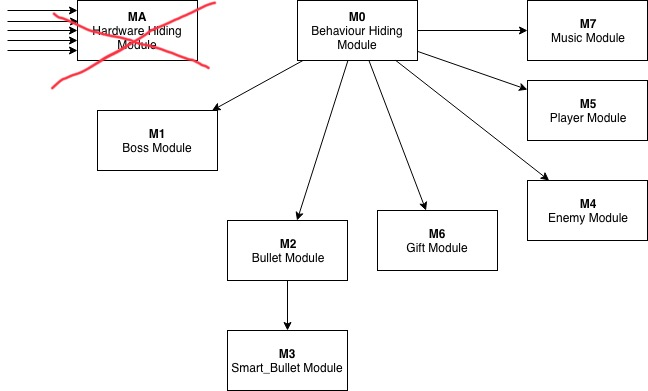
\includegraphics[scale=0.74]{moduleHierarchy}
\bigbreak
Figure 1: Uses hierarchy between modules

\section{Schedule}

\subsection{Gantt}
	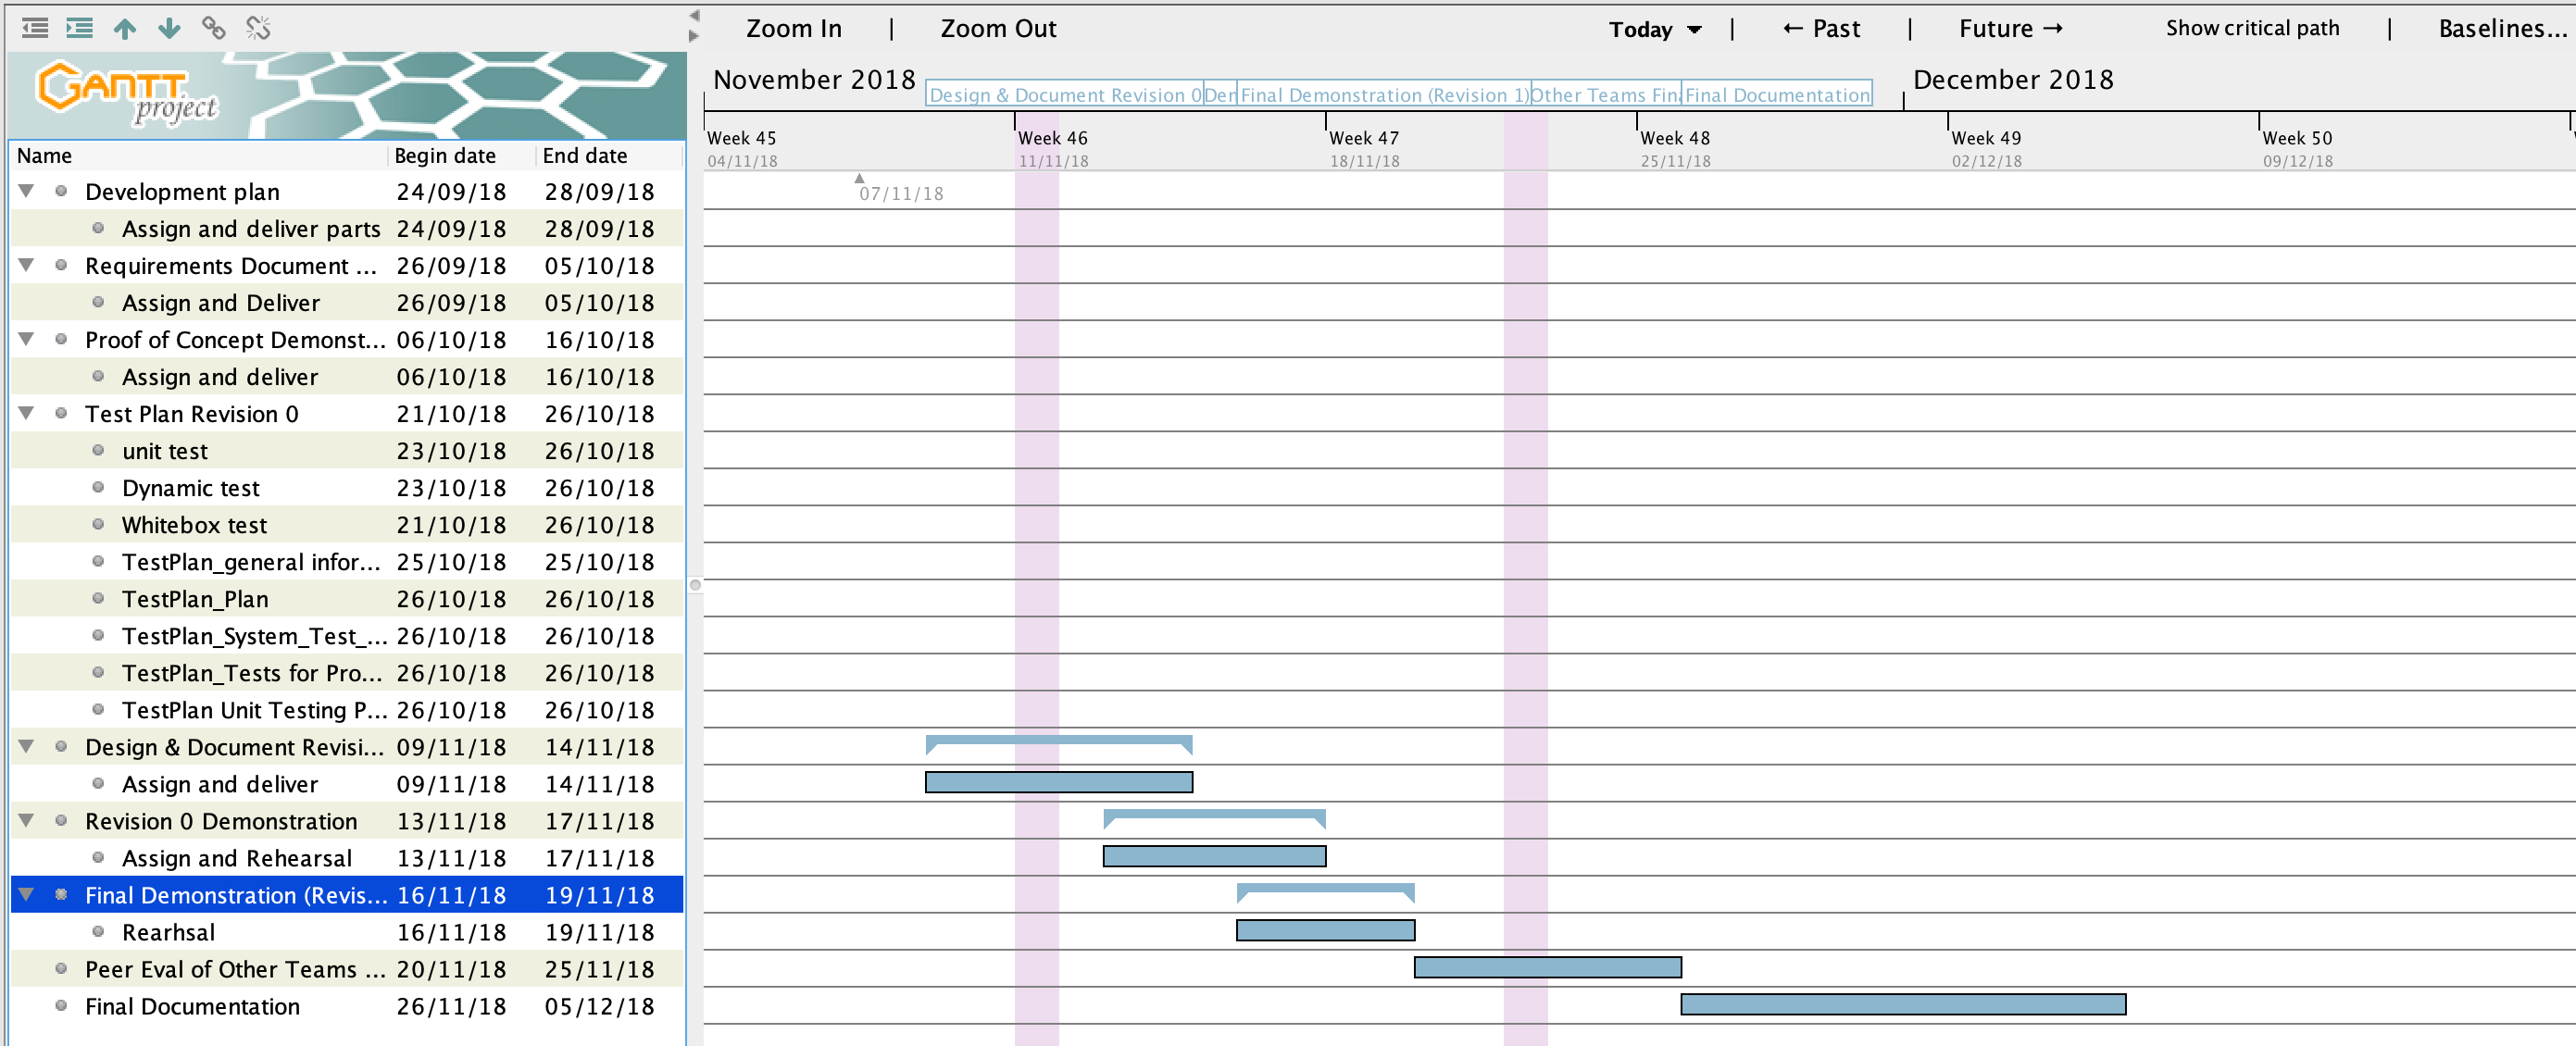
\includegraphics[scale=0.32]{Gantt.png}
	
	Figure 2: Gantt chart of project schedule
	
\section{Major Revision History}
November 7, 2018 - Rough draft of sections\\
November 8, 2018 - Revised sections\\ 
November 9, 2018 - Revision 0 complete\\
December 5, 2018 - Revision 1 complete

\bibliography{bib}
\bibliographystyle{plain}
\end{document}